\chapter{Properties}
\label{Properties}

\paragraph{}
In this chapter we discuss the implications of what we have seen in the previous chapter, in particular the implications of Property~\ref{intersection-patterns}. We start with a direct consequence of the definition of a permutation representation graph.

\begin{proposition}
  \label{fixed-only-1}
  In a permutation representation graph, two edges with the same index cannot be adjacent.
\end{proposition}

\begin{proof}
  Here is one graph of this situation:

  \begin{figure}[H]
    \begin{center}
      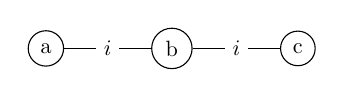
\begin{tikzpicture}[scale=.8]

        \begin{scope}[every node/.style={circle,draw, transform shape}]
          \node (1)  at (0,0)  {a};
          \node (2)  at (2,0)  {b};
          \node (3)  at (4,0)  {c};
        \end{scope}

        \begin{scope}[every node/.style={fill=white, transform shape}]

          \begin{scope}[every edge/.style={draw}]
            \path (1)  edge node {$i$} (2);
            \path (2)  edge node {$i$} (3);
          \end{scope}
        \end{scope}

      \end{tikzpicture}
      \caption{}
    \end{center}
  \end{figure}

  \paragraph{}
  If a such graph exists, there is an edge labeled with $i$ between $a$ and $b$ thus, by definition of a permutation representation graph, $a \rho_i = b$ and $b \rho_i = a$. There is also an edge labeled with $i$ between $b$ and $c$, thus $b \rho_i = c$ and $c \rho_i = b$. There is a contradiction because $a = b \rho_i = c$ but $a \neq c$. Thus this graph is impossible.
\end{proof}

\paragraph{}
We define three patterns that are used in the construction of permutation representation graphs.

\section{Definitions}
\begin{definition}[Alternating square]
  \index{alternating square}
  An alternating square is a set of 4 vertices and 4 edges that form the following graph:

  \begin{figure}[H]
    \begin{center}
      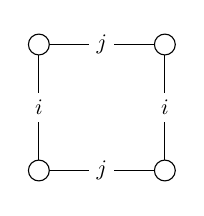
\begin{tikzpicture}[scale=.8]

        \begin{scope}[every node/.style={circle,draw, transform shape}]
          \node (1)  at (0,2)  {};
          \node (2)  at (0,0)  {};
          \node (3)  at (2,2)  {};
          \node (4)  at (2,0)  {};
        \end{scope}

        \begin{scope}[every node/.style={fill=white, transform shape}]

          \begin{scope}[every edge/.style={draw}]
            \path (1)  edge node {$i$} (2);
            \path (3)  edge node {$i$} (4);
            \path (1)  edge node {$j$} (3);
            \path (2)  edge node {$j$} (4);
          \end{scope}
        \end{scope}

      \end{tikzpicture}
      \caption{}
    \end{center}
  \end{figure}

  \paragraph{}
  Additional edges can be present on the permutation representation graph even between vertices of the alternating square.

  \paragraph{}
  This alternating square is denoted $[\rho_i, \rho_j]$.
\end{definition}

\begin{definition}[Multiple edge]
  \index{multiple edge}
  \index{double edge}

  A \textit{multiple edge} is a pair of vertices and a set of at least two edges linking those vertices. The number of edges is called the multiplicity of the multiple edge. If the multiplicity is exactly two, it is called a \textit{double edge}.

  \begin{figure}[H]
    \begin{center}
      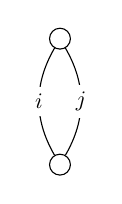
\begin{tikzpicture}[scale=.8]

        \begin{scope}[every node/.style={circle,draw, transform shape}]
          \node (1)  at (0,2)  {};
          \node (2)  at (0,0)  {};
        \end{scope}

        \begin{scope}[every node/.style={fill=white, transform shape}]

          \begin{scope}[every edge/.style={draw}]
            \path (1)  edge[bend right=30] node {$i$} (2);
            \path (1)  edge[bend left=30] node {$j$} (2);
          \end{scope}
        \end{scope}

      \end{tikzpicture}
      \caption{}
    \end{center}
  \end{figure}

  \paragraph{}
  A double edge is denoted $(\rho_i, \rho_j)$.
\end{definition}

\begin{definition}[Single edge]
  \label{single-edge}
  \index{single-edge}
  A single edge is a pair of vertices and an edge such that both vertices are not in the same alternating square or in the same multiple edge.
\end{definition}

\paragraph{}
Note that the word \textit{edge} without adjectives conserves its original meaning of the graph theory. We only define a special type of edges in this section.

\paragraph{}
Now we continue with the implications on the permutation representation graphs.

\section{Single edges}

\begin{definition}
  An edge (single or multiple) is called adjacent to another pattern if they share exactly one vertex.
\end{definition}

\paragraph{}
If a single edge shares more than one vertex with a given pattern then it is not a single edge by Definition~\ref{single-edge}.

\begin{definition}
  A sequence of adjacent single edges is called a chain.
\end{definition}

\begin{proposition}
  \label{chain-consecutive}
  In a chain, the indices of two adjacent edges must be consecutive.
\end{proposition}

\begin{proof}
  The situation is this graph:

  \begin{figure}[H]
    \begin{center}
      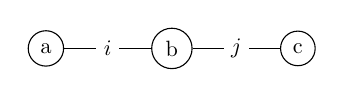
\begin{tikzpicture}[scale=.8]

        \begin{scope}[every node/.style={circle,draw, transform shape}]
          \node (1)  at (0,0)  {a};
          \node (2)  at (2,0)  {b};
          \node (3)  at (4,0)  {c};
        \end{scope}

        \begin{scope}[every node/.style={fill=white, transform shape}]

          \begin{scope}[every edge/.style={draw}]
            \path (1)  edge node {$i$} (2);
            \path (2)  edge node {$j$} (3);
          \end{scope}
        \end{scope}

      \end{tikzpicture}
      \caption{}
    \end{center}
  \end{figure}

  \paragraph{}
  If $i$ and $j$ are not consecutive, the graph obtained from the permutation representation graph where only the $\rho_i$ and $\rho_j$ edges are kept must only form the patterns displayed in Property~\ref{intersection-patterns}.

  \paragraph{}
  The pattern of the graph cannot form fixed points, distinct single edges or a double edge. Thus the only remaining pattern of Property~\ref{intersection-patterns} is the alternating square. But if those two edges are part of an alternating square, there are no more single edges and thus they do not form a chain which is a contradiction.

  \paragraph{}
  Thus in a chain, the indices must be consecutive.
\end{proof}

\section{Multiple edges}

\begin{proposition}
  A multiple edge with multiplicity three or more cannot be connected to a single edge.
\end{proposition}

\begin{proof}
  Let $\Gamma$ be the graph representing the situation:

  \begin{figure}[H]
    \begin{center}
      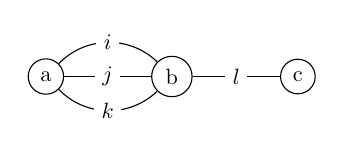
\begin{tikzpicture}[scale=.8]

        \begin{scope}[every node/.style={circle,draw, transform shape}]
          \node (1)  at (0,0)  {a};
          \node (2)  at (2,0)  {b};
          \node (3)  at (4,0)  {c};
        \end{scope}

        \begin{scope}[every node/.style={fill=white, transform shape}]

          \begin{scope}[every edge/.style={draw}]
            \path (1)  edge[bend left=45] node {$i$} (2);
            \path (1)  edge node {$j$} (2);
            \path (1)  edge[bend right=45] node {$k$} (2);
            \path (2)  edge node {$l$} (3);
          \end{scope}
        \end{scope}

      \end{tikzpicture}
      \caption{}
    \end{center}
  \end{figure}

  \paragraph{}
  In this situation $i,j,k$ and $l$ are different by Proposition~\ref{fixed-only-1}. Therefore there exists an edge, suppose $k$, such that $|k - l| > 1$. Thus $\rho_i$ and $\rho_l$ must commute. But there is a chain of length 2 with non consecutive indices in the graph $\Gamma_{\rho_i \rho_l}$ which is impossible by Proposition~\ref{chain-consecutive}.
\end{proof}

\begin{definition}
  A double edge is included into an alternating square if both vertices of the double edge are vertices of the alternating square.
\end{definition}

\begin{proposition}
  A multiple edge that is not included in an alternating square cannot be adjacent to either an alternating square or another double edge.
\end{proposition}

\begin{proof}
  The proof of this proposition is similar to the previous one. Here is the graph of $\Gamma$.

  \begin{figure}[H]
    \begin{center}
      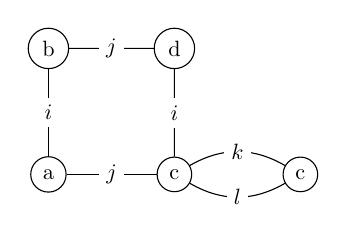
\begin{tikzpicture}[scale=.8]

        \begin{scope}[every node/.style={circle,draw, transform shape}]
          \node (1)  at (0,0)  {a};
          \node (2)  at (0,2)  {b};
          \node (3)  at (2,0)  {c};
          \node (4)  at (2,2)  {d};
          \node (5)  at (4,0)  {c};
        \end{scope}

        \begin{scope}[every node/.style={fill=white, transform shape}]

          \begin{scope}[every edge/.style={draw}]
            \path (1)  edge node {$i$} (2);
            \path (3)  edge node {$i$} (4);
            \path (1)  edge node {$j$} (3);
            \path (2)  edge node {$j$} (4);
            \path (3)  edge[bend left=30] node {$k$} (5);
            \path (3)  edge[bend right=30] node {$l$} (5);
          \end{scope}
        \end{scope}

      \end{tikzpicture}
      \caption{}
    \end{center}
  \end{figure}

  \paragraph{}
  Here there exists a pair, suppose $j$ and $l$ such that $|j-l| > 1$. Thus, in $\Gamma_{\rho_j, \rho_l}$, there is a chain of length 2. An alternating square must thus be built but that is a contradiction.

  \paragraph{}
  The same applies for two adjacent double edges.

\end{proof}

\begin{proposition}
  \label{adjacent-double}
  A double edge $(\rho_i, \rho_j)$ can only be adjacent to a single edge if the difference between the indices of its edges is exactly 2. In this case the index of the single edge must be in the middle of the indices of the double edge i.e. if the index of the single edge is $k$ then $|i-k| = 1$ and $|j-k| = 1$.
\end{proposition}

\begin{proof}
  This can be clearly deduced from the graph:

  \begin{figure}[H]
    \begin{center}
      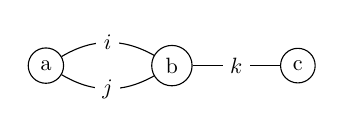
\begin{tikzpicture}[scale=.8]

        \begin{scope}[every node/.style={circle,draw, transform shape}]
          \node (1)  at (0,0)  {a};
          \node (2)  at (2,0)  {b};
          \node (3)  at (4,0)  {c};
        \end{scope}

        \begin{scope}[every node/.style={fill=white, transform shape}]

          \begin{scope}[every edge/.style={draw}]
            \path (1)  edge[bend left=30] node {$i$} (2);
            \path (1)  edge[bend right=30] node {$j$} (2);
            \path (2)  edge node {$k$} (3);
          \end{scope}
        \end{scope}

      \end{tikzpicture}
      \caption{}
    \end{center}
  \end{figure}

  The indices $i$ and $k$ must be consecutive, but $k$ and $j$ must also be consecutive. That leads immediately to the conclusion.

\end{proof}

\begin{corollary}
  \label{continue-double-edge}
  Let $(\rho_i, \rho_j)$ be a double edge. If $|i - j| \neq 2$ then the double edge must be included into an alternating square. Furthermore the alternating square must be  $[\rho_{i-1}, \rho_j]$, $[\rho_{i+1}, \rho_j]$, $[\rho_i, \rho_{j-1}]$ or $[\rho_i, \rho_{j+1}]$.
\end{corollary}

\begin{proposition}
  \label{continue-triple-edge}
  A triple edge or a quadruple edge can only be connected if it is included in an alternating square.
\end{proposition}

\section{Alternating squares}

\paragraph{}
In an alternating square $[\rho_i, \rho_j]$ we call $\rho_i$ and $\rho_j$ the \textit{components} of the alternating square.

\begin{proposition}
  \label{square-connection}
  Given an alternating square $[\rho_i, \rho_j]$ a single edge can be adjacent to this square only if $|i - j| = 2$. In this case the index of the single edge is in in the middle of the two indices i.e. if the index of the edge is $k$ then $|i-k| = 1$ and $|j-k| = 1$.
\end{proposition}

\begin{definition}
  Two alternating squares are adjacent if they share two vertices.
\end{definition}

\begin{proposition}
  \label{adjacent-squares}
  Given an alternating square $[\rho_i, \rho_j]$ the only possible adjacent alternating squares are $[\rho_{i-1}, \rho_j], [\rho_{i+1}, \rho_j], [\rho_i, \rho_{j-1}]$ or $[\rho_i, \rho_{j+1}]$ if the intersection of both square is a single edge.
\end{proposition}

\begin{corollary}
  \label{continue-alternating-square}
  If the difference between the indices of an alternating square is not 2, then this square must be adjacent to another alternating square.
\end{corollary}

\begin{corollary}
  If two alternating squares are adjacent and their intersection is a single edge, then they share a component and the difference between the indices of the other component is exactly 1.
\end{corollary}

\paragraph{}
Due to the fact that some alternating squares must be adjacent to other ones, we will deal with sequence of alternating squares.

\begin{definition}[Sequence of alternating squares]
  \index{sequence of alternating squares}
  A \textit{sequence of alternating squares} is a sequence such that two consecutive squares are adjacent.
\end{definition}

\begin{definition}[Non-cyclic sequence of alternating squares]
  \index{Non-cyclic sequence of atlernating squares}
  A \textit{non-cyclic sequence of alternating squares} is a sequence of alternating squares such that no squares appear multiple times in the sequence.
\end{definition}

\begin{definition}[Cyclic sequence of alternating squares]
  \index{cycle (permutation representation graph)}
  \index{cyclic sequence of alternating squares}
  A \textit{cyclic sequence of alternating squares} or \textit{cycle} is a sequence of alternating squares such that at least one square appears multiple times in the sequence.
\end{definition}

\begin{definition}[Simple cycle]
  \index{simple cycle}
  A cycle is said \textit{simple} if the first and the last squares of the sequence are the same.
\end{definition}

\begin{corollary}
  \label{cycle-simple-cycle}
  Every cycle contains a simple cycle and thus if a permutation representation graph does not contain any simple cycle, it does not contain any cycle.
\end{corollary}

\begin{definition}[Linear sequence of alternating squares]
    A sequence of alternating square is said \textit{linear} if two alternating squares that are not consecutive does not share any vertex.
\end{definition}

\begin{definition}[Monotone sequence of alternating squares]
  \index{monotone sequence of alternating squares}
  A linear sequence of alternating square is said \textit{monotone} if all alternating squares have one common component.
\end{definition}

\begin{proposition}
  \label{parity-sequence-squares}
  If an alternating square in a linear monotone sequence can be connected to a single edge then the number of squares that must be added to the sequence such that is can be connected is even.
\end{proposition}

\begin{proof}
  This can be deduced from Proposition~\ref{sequence-connection} and~\ref{adjacent-squares}.
\end{proof}

\begin{proposition}
  \label{rotation-pattern}
  If a sequence of alternating squares is not linear, then it contains a simple cycle of 4 squares or it contains the following pattern.

  \begin{figure}[H]
    \begin{center}
      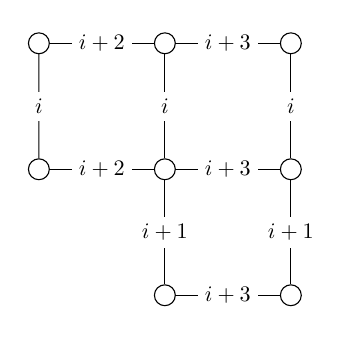
\begin{tikzpicture}[scale=.8]

        \begin{scope}[every node/.style={circle,draw, transform shape}]
          \node (1)  at (0,2)  {};
          \node (2)  at (0,0)  {};
          \node (3)  at (0,-2) {};
          \node (4)  at (-2,2)  {};
          \node (5)  at (-2,0)  {};
          \node (6)  at (-2,-2) {};
          \node (7)  at (-4,2)  {};
          \node (8)  at (-4,0)  {};
        \end{scope}

        \begin{scope}[every node/.style={fill=white, transform shape}]

          \begin{scope}[every edge/.style={draw}]
            \path (2)  edge node {$i+1$} (3);
            \path (5)  edge node {$i+1$} (6);
            \path (1)  edge node {$i$} (2);
            \path (4)  edge node {$i$} (5);
            \path (7)  edge node {$i$} (8);
            \path (1)  edge node {$i+3$} (4);
            \path (2)  edge node {$i+3$} (5);
            \path (3)  edge node {$i+3$} (6);
            \path (4)  edge node {$i+2$} (7);
            \path (5)  edge node {$i+2$} (8);
          \end{scope}
        \end{scope}

      \end{tikzpicture}
      \caption{}
    \end{center}
  \end{figure}
\end{proposition}

\begin{proof}
  we start with four different indices $i, j, k, l$ and two squares that share exactly one vertex.

  \begin{figure}[H]
    \begin{center}
      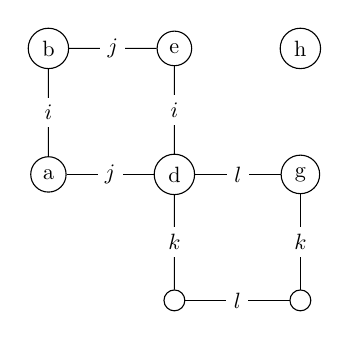
\begin{tikzpicture}[scale=.8]

        \begin{scope}[every node/.style={circle,draw, transform shape}]
          \node (1)  at (0,2)  {h};
          \node (2)  at (0,0)  {g};
          \node (3)  at (0,-2) {};
          \node (4)  at (-2,2)  {e};
          \node (5)  at (-2,0)  {d};
          \node (6)  at (-2,-2) {};
          \node (7)  at (-4,2)  {b};
          \node (8)  at (-4,0)  {a};
        \end{scope}

        \begin{scope}[every node/.style={fill=white, transform shape}]

          \begin{scope}[every edge/.style={draw}]
            \path (2)  edge node {$k$} (3);
            \path (5)  edge node {$k$} (6);
            \path (4)  edge node {$i$} (5);
            \path (7)  edge node {$i$} (8);
            \path (2)  edge node {$l$} (5);
            \path (3)  edge node {$l$} (6);
            \path (4)  edge node {$j$} (7);
            \path (5)  edge node {$j$} (8);
          \end{scope}
        \end{scope}

      \end{tikzpicture}
      \caption{}
    \end{center}
  \end{figure}

  \paragraph{}
  But there is a problem at the point $d$ because it is impossible that both indices of $(i,j)$ commutes with both indices of $(k,l)$. Thus there must be at least one pair of non consecutive indices. Suppose that it is $(i,l)$, the other cases are isomorphic. An alternating square must be built to include the edges $(e,d)$ and $(d,g)$.

  \paragraph{}
  The last vertex of the square can be $a$, $b$ or $h$ up to isomorphim. That makes no sense to use $a$ or $b$ because if an alternating square $[\rho_i, \rho_l]$ is built on the points $a,e,d,g$ then there is a $\rho_i$ edge between $a$ and $g$ and $a$ is already linked to $b$ by a $\rho_i$ edge, thus this is impossible by Proposition~\ref{fixed-only-1}. The same applies to $b$, hence the alternating square between $\rho_i$ and $\rho_l$ must use the vertex $h$.

  \begin{figure}[H]
    \begin{center}
      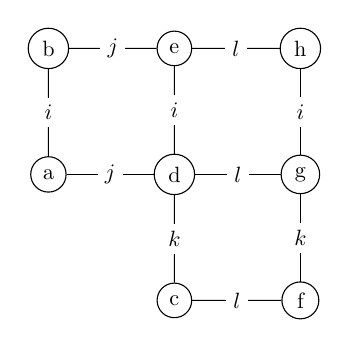
\begin{tikzpicture}[scale=.8]

        \begin{scope}[every node/.style={circle,draw, transform shape}]
          \node (1)  at (0,2)  {h};
          \node (2)  at (0,0)  {g};
          \node (3)  at (0,-2) {f};
          \node (4)  at (-2,2)  {e};
          \node (5)  at (-2,0)  {d};
          \node (6)  at (-2,-2) {c};
          \node (7)  at (-4,2)  {b};
          \node (8)  at (-4,0)  {a};
        \end{scope}

        \begin{scope}[every node/.style={fill=white, transform shape}]

          \begin{scope}[every edge/.style={draw}]
            \path (2)  edge node {$k$} (3);
            \path (5)  edge node {$k$} (6);
            \path (1)  edge node {$i$} (2);
            \path (4)  edge node {$i$} (5);
            \path (7)  edge node {$i$} (8);
            \path (1)  edge node {$l$} (4);
            \path (2)  edge node {$l$} (5);
            \path (3)  edge node {$l$} (6);
            \path (4)  edge node {$j$} (7);
            \path (5)  edge node {$j$} (8);
          \end{scope}
        \end{scope}

      \end{tikzpicture}
      \caption{}
    \end{center}
  \end{figure}

  \paragraph{}
  Suppose now that $j$ and $k$ are not consecutive, then another alternating square must be built on the points $a,c,d$. This square must use a new point. The graph is now:

  \begin{figure}[H]
    \begin{center}
      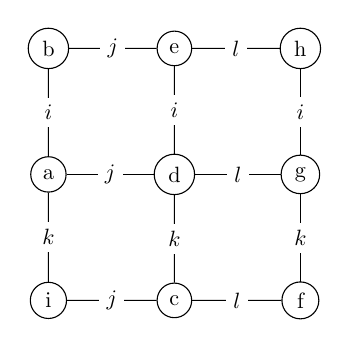
\begin{tikzpicture}[scale=.8]

        \begin{scope}[every node/.style={circle,draw, transform shape}]
          \node (1)  at (0,2)  {h};
          \node (2)  at (0,0)  {g};
          \node (3)  at (0,-2) {f};
          \node (4)  at (-2,2)  {e};
          \node (5)  at (-2,0)  {d};
          \node (6)  at (-2,-2) {c};
          \node (7)  at (-4,2)  {b};
          \node (8)  at (-4,0)  {a};
          \node (9)  at (-4,-2)  {i};
        \end{scope}

        \begin{scope}[every node/.style={fill=white, transform shape}]

          \begin{scope}[every edge/.style={draw}]
            \path (2)  edge node {$k$} (3);
            \path (5)  edge node {$k$} (6);
            \path (8)  edge node {$k$} (9);
            \path (1)  edge node {$i$} (2);
            \path (4)  edge node {$i$} (5);
            \path (7)  edge node {$i$} (8);
            \path (1)  edge node {$l$} (4);
            \path (2)  edge node {$l$} (5);
            \path (3)  edge node {$l$} (6);
            \path (4)  edge node {$j$} (7);
            \path (5)  edge node {$j$} (8);
            \path (6)  edge node {$j$} (9);
          \end{scope}
        \end{scope}

      \end{tikzpicture}
      \caption{}
    \end{center}
  \end{figure}

  \paragraph{}
  There is a cycle of 4 squares in this graph. Otherwise $j$ and $k$ must be consecutive, thus $j = k+1$ up to duality.

  \begin{figure}[H]
    \begin{center}
      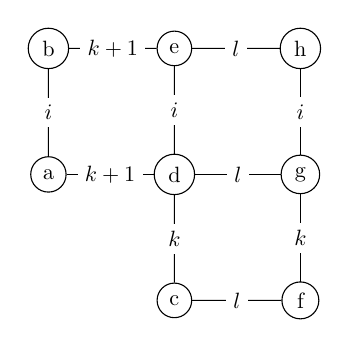
\begin{tikzpicture}[scale=.8]

        \begin{scope}[every node/.style={circle,draw, transform shape}]
          \node (1)  at (0,2)  {h};
          \node (2)  at (0,0)  {g};
          \node (3)  at (0,-2) {f};
          \node (4)  at (-2,2)  {e};
          \node (5)  at (-2,0)  {d};
          \node (6)  at (-2,-2) {c};
          \node (7)  at (-4,2)  {b};
          \node (8)  at (-4,0)  {a};
        \end{scope}

        \begin{scope}[every node/.style={fill=white, transform shape}]

          \begin{scope}[every edge/.style={draw}]
            \path (2)  edge node {$k$} (3);
            \path (5)  edge node {$k$} (6);
            \path (1)  edge node {$i$} (2);
            \path (4)  edge node {$i$} (5);
            \path (7)  edge node {$i$} (8);
            \path (1)  edge node {$l$} (4);
            \path (2)  edge node {$l$} (5);
            \path (3)  edge node {$l$} (6);
            \path (4)  edge node {$k+1$} (7);
            \path (5)  edge node {$k+1$} (8);
          \end{scope}
        \end{scope}

      \end{tikzpicture}
      \caption{}
    \end{center}
  \end{figure}

  \paragraph{}
  Suppose now that $i$ and $k$ are not consecutive, then two alternating squares must be built on $c,d,e$ and $f,g,h$. None of those squares can use existing points. The graph is the following:

  \begin{figure}[H]
    \begin{center}
      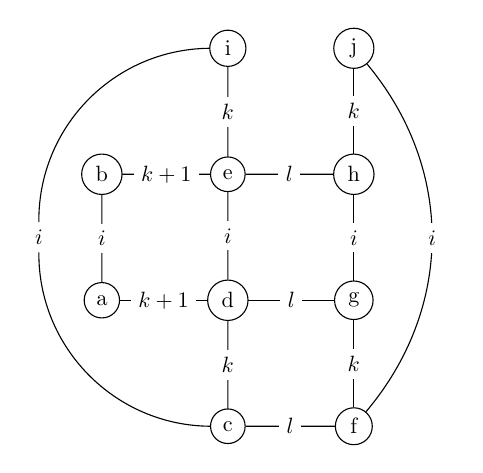
\begin{tikzpicture}[scale=.8]

        \begin{scope}[every node/.style={circle,draw, transform shape}]
          \node (1)  at (0,2)  {h};
          \node (2)  at (0,0)  {g};
          \node (3)  at (0,-2) {f};
          \node (4)  at (-2,2)  {e};
          \node (5)  at (-2,0)  {d};
          \node (6)  at (-2,-2) {c};
          \node (7)  at (-4,2)  {b};
          \node (8)  at (-4,0)  {a};
          \node (9)  at (-2,4)  {i};
          \node (10) at (0,4)   {j};
        \end{scope}

        \begin{scope}[every node/.style={fill=white, transform shape}]

          \node (t) at (-5,1)   {$i$};

          \begin{scope}[every edge/.style={draw}]
            \path (2)  edge node {$k$} (3);
            \path (5)  edge node {$k$} (6);
            \path (9)  edge node {$k$} (4);
            \path (10) edge node {$k$} (1);
            \path (1)  edge node {$i$} (2);
            \path (4)  edge node {$i$} (5);
            \path (7)  edge node {$i$} (8);
            \path (9)  edge[bend right=45] (t);
            \path (t)  edge[bend right=45] (6);
            \path (10) edge[bend left=40] node {$i$} (3);
            \path (1)  edge node {$l$} (4);
            \path (2)  edge node {$l$} (5);
            \path (3)  edge node {$l$} (6);
            \path (4)  edge node {$k+1$} (7);
            \path (5)  edge node {$k+1$} (8);
          \end{scope}
        \end{scope}

      \end{tikzpicture}
      \caption{}
    \end{center}
  \end{figure}

  \paragraph{}
  Now if $i$ and $l$ are not consecutive then a $\rho_l$ edge must be added between the points $i$ and $j$. This edge form a cycle of four alternating squares. Therefore $i$ and $l$ must commute and $l = i+1$. Moreover the same applies to $k$ and $i+1$, thus $k = i + 2$.

  \begin{figure}[H]
    \begin{center}
      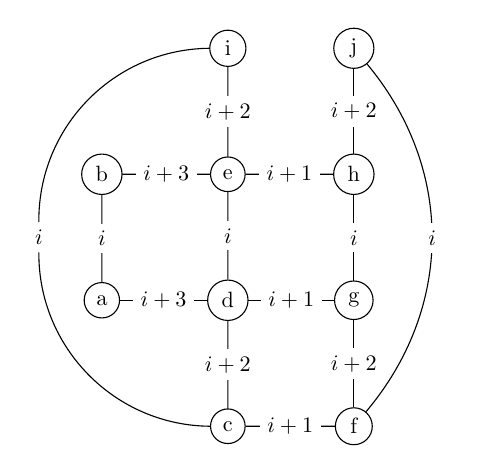
\begin{tikzpicture}[scale=.8]

        \begin{scope}[every node/.style={circle,draw, transform shape}]
          \node (1)  at (0,2)  {h};
          \node (2)  at (0,0)  {g};
          \node (3)  at (0,-2) {f};
          \node (4)  at (-2,2)  {e};
          \node (5)  at (-2,0)  {d};
          \node (6)  at (-2,-2) {c};
          \node (7)  at (-4,2)  {b};
          \node (8)  at (-4,0)  {a};
          \node (9)  at (-2,4)  {i};
          \node (10) at (0,4)   {j};
        \end{scope}

        \begin{scope}[every node/.style={fill=white, transform shape}]

          \node (t) at (-5,1)   {$i$};

          \begin{scope}[every edge/.style={draw}]
            \path (2)  edge node {$i+2$} (3);
            \path (5)  edge node {$i+2$} (6);
            \path (9)  edge node {$i+2$} (4);
            \path (10) edge node {$i+2$} (1);
            \path (1)  edge node {$i$} (2);
            \path (4)  edge node {$i$} (5);
            \path (7)  edge node {$i$} (8);
            \path (9)  edge[bend right=45] (t);
            \path (t)  edge[bend right=45] (6);
            \path (10) edge[bend left=40] node {$i$} (3);
            \path (1)  edge node {$i+1$} (4);
            \path (2)  edge node {$i+1$} (5);
            \path (3)  edge node {$i+1$} (6);
            \path (4)  edge node {$i+3$} (7);
            \path (5)  edge node {$i+3$} (8);
          \end{scope}
        \end{scope}

      \end{tikzpicture}
      \caption{}
    \end{center}
  \end{figure}

  \paragraph{}
  There is the same problem in the horizontal direction. Thus two other alternating squares must be built on $b, e, h$ and $a, d, g$ because $\rho_{i+1}$ and $\rho_{i+3}$ does not commute.

  \begin{figure}[H]
    \begin{center}
      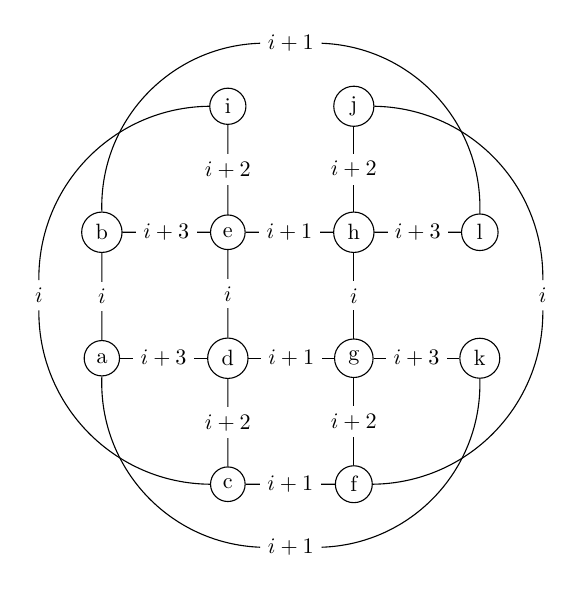
\begin{tikzpicture}[scale=.8]

        \begin{scope}[every node/.style={circle,draw, transform shape}]
          \node (1)  at (0,2)  {h};
          \node (2)  at (0,0)  {g};
          \node (3)  at (0,-2) {f};
          \node (4)  at (-2,2)  {e};
          \node (5)  at (-2,0)  {d};
          \node (6)  at (-2,-2) {c};
          \node (7)  at (-4,2)  {b};
          \node (8)  at (-4,0)  {a};
          \node (9)  at (-2,4)  {i};
          \node (10) at (0,4)   {j};
          \node (11) at (2,0)   {k};
          \node (12) at (2,2)   {l};
        \end{scope}

        \begin{scope}[every node/.style={fill=white, transform shape}]

          \node (t1) at (-5,1)  {$i$};
          \node (t2) at (3,1)   {$i$};
          \node (t3) at (-1,-3) {$i+1$};
          \node (t4) at (-1,5)  {$i+1$};

          \begin{scope}[every edge/.style={draw}]
            \path (2)  edge node {$i+2$} (3);
            \path (5)  edge node {$i+2$} (6);
            \path (9)  edge node {$i+2$} (4);
            \path (10) edge node {$i+2$} (1);
            \path (1)  edge node {$i$} (2);
            \path (4)  edge node {$i$} (5);
            \path (7)  edge node {$i$} (8);
            \path (9)  edge[bend right=45] (t1);
            \path (t1) edge[bend right=45] (6);
            \path (10) edge[bend left=45] (t2);
            \path (t2) edge[bend left=45] (3);
            \path (12) edge[bend right=45] (t4);
            \path (t4) edge[bend right=45] (7);
            \path (11) edge[bend left=45] (t3);
            \path (t3) edge[bend left=45] (8);
            \path (1)  edge node {$i+1$} (4);
            \path (2)  edge node {$i+1$} (5);
            \path (3)  edge node {$i+1$} (6);
            \path (4)  edge node {$i+3$} (7);
            \path (5)  edge node {$i+3$} (8);
            \path (1)  edge node {$i+3$} (12);
            \path (2)  edge node {$i+3$} (11);
          \end{scope}
        \end{scope}

      \end{tikzpicture}
      \caption{}
    \end{center}
  \end{figure}

  \paragraph{}
  A $\rho_i$ edge must be placed between $k$ and $l$ because $\rho_i$ and $\rho_{i+3}$ does not commute. Thus there is a cycle of four squares.

  \paragraph{}
  We choose that $i$ and $k$ are not consecutive and we only make cycles. The graph was this:

  \begin{figure}[H]
    \begin{center}
      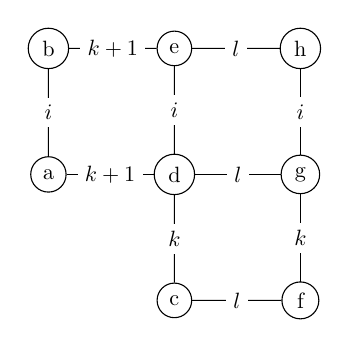
\begin{tikzpicture}[scale=.8]

        \begin{scope}[every node/.style={circle,draw, transform shape}]
          \node (1)  at (0,2)  {h};
          \node (2)  at (0,0)  {g};
          \node (3)  at (0,-2) {f};
          \node (4)  at (-2,2)  {e};
          \node (5)  at (-2,0)  {d};
          \node (6)  at (-2,-2) {c};
          \node (7)  at (-4,2)  {b};
          \node (8)  at (-4,0)  {a};
        \end{scope}

        \begin{scope}[every node/.style={fill=white, transform shape}]

          \begin{scope}[every edge/.style={draw}]
            \path (2)  edge node {$k$} (3);
            \path (5)  edge node {$k$} (6);
            \path (1)  edge node {$i$} (2);
            \path (4)  edge node {$i$} (5);
            \path (7)  edge node {$i$} (8);
            \path (1)  edge node {$l$} (4);
            \path (2)  edge node {$l$} (5);
            \path (3)  edge node {$l$} (6);
            \path (4)  edge node {$k+1$} (7);
            \path (5)  edge node {$k+1$} (8);
          \end{scope}
        \end{scope}

      \end{tikzpicture}
      \caption{}
    \end{center}
  \end{figure}

  \paragraph{}
  Now we look at the case were $i$ and $k$ are consecutive i.e. $k = i+1$ up to duality. By isomorphim the same applies to $k+1$ and $l$ and thus $l = k+1 = i+2$.

  \begin{figure}[H]
    \begin{center}
      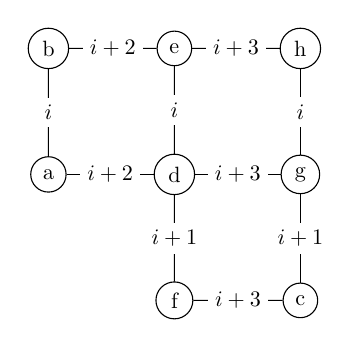
\begin{tikzpicture}[scale=.8]

        \begin{scope}[every node/.style={circle,draw, transform shape}]
          \node (1)  at (0,2)  {h};
          \node (2)  at (0,0)  {g};
          \node (3)  at (0,-2) {c};
          \node (4)  at (-2,2)  {e};
          \node (5)  at (-2,0)  {d};
          \node (6)  at (-2,-2) {f};
          \node (7)  at (-4,2)  {b};
          \node (8)  at (-4,0)  {a};
        \end{scope}

        \begin{scope}[every node/.style={fill=white, transform shape}]

          \begin{scope}[every edge/.style={draw}]
            \path (2)  edge node {$i+1$} (3);
            \path (5)  edge node {$i+1$} (6);
            \path (1)  edge node {$i$} (2);
            \path (4)  edge node {$i$} (5);
            \path (7)  edge node {$i$} (8);
            \path (1)  edge node {$i+3$} (4);
            \path (2)  edge node {$i+3$} (5);
            \path (3)  edge node {$i+3$} (6);
            \path (4)  edge node {$i+2$} (7);
            \path (5)  edge node {$i+2$} (8);
          \end{scope}
        \end{scope}

      \end{tikzpicture}
      \caption{}
    \end{center}
  \end{figure}

  \paragraph{}
  And this is the pattern of the statement.

\end{proof}

\begin{corollary}
  Every linear cycle contains an even number of points.
\end{corollary}


\begin{proposition}
  \label{linear-pattern}
  On a polytope of rank 5 or less, every non-monotone linear sequence of alternating squares contains one cycle with three squares or one of the two following patterns:

  \begin{figure}[H]
    \begin{center}
      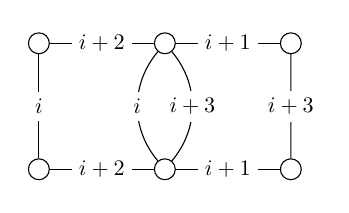
\begin{tikzpicture}[scale=.8]

        \begin{scope}[every node/.style={circle,draw, transform shape}]
          \node (1)  at (0,2)  {};
          \node (2)  at (0,0)  {};
          \node (3)  at (2,2)  {};
          \node (4)  at (2,0)  {};
          \node (5)  at (4,2)  {};
          \node (6)  at (4,0)  {};
        \end{scope}

        \begin{scope}[every node/.style={fill=white, transform shape}]

          \begin{scope}[every edge/.style={draw}]
            \path (1)  edge node {$i$} (2);
            \path (3)  edge[bend right=40] node {$i$} (4);
            \path (1)  edge node {$i+2$} (3);
            \path (2)  edge node {$i+2$} (4);
            \path (3)  edge node {$i+1$} (5);
            \path (4)  edge node {$i+1$} (6);
            \path (3)  edge[bend left=40] node {$i+3$} (4);
            \path (5)  edge node {$i+3$} (6);

          \end{scope}
        \end{scope}

      \end{tikzpicture}
      \caption{}
      \label{linear-1}
    \end{center}
  \end{figure}

  \begin{figure}[H]
    \begin{center}
      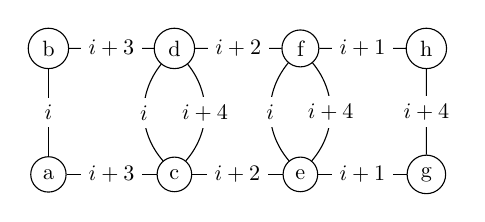
\begin{tikzpicture}[scale=.8]

        \begin{scope}[every node/.style={circle,draw, transform shape}]
          \node (1)  at (0,2)  {b};
          \node (2)  at (0,0)  {a};
          \node (3)  at (2,2)  {d};
          \node (4)  at (2,0)  {c};
          \node (5)  at (4,2)  {f};
          \node (6)  at (4,0)  {e};
          \node (7)  at (6,2)  {h};
          \node (8)  at (6,0)  {g};
        \end{scope}

        \begin{scope}[every node/.style={fill=white, transform shape}]

          \begin{scope}[every edge/.style={draw}]
            \path (1)  edge node {$i$} (2);
            \path (3)  edge[bend right=40] node {$i$} (4);
            \path (5)  edge[bend right=40] node {$i$} (6);
            \path (1)  edge node {$i+3$} (3);
            \path (2)  edge node {$i+3$} (4);
            \path (3)  edge node {$i+2$} (5);
            \path (4)  edge node {$i+2$} (6);
            \path (7)  edge node {$i+1$} (5);
            \path (8)  edge node {$i+1$} (6);
            \path (3)  edge[bend left=40] node {$i+4$} (4);
            \path (5)  edge[bend left=40] node {$i+4$} (6);
            \path (7)  edge node {$i+4$} (8);

          \end{scope}
        \end{scope}

      \end{tikzpicture}
      \caption{}
    \end{center}
  \end{figure}

\end{proposition}

\begin{proof}
  We have two adjacents alternating squares that do not share a component, thus the common edge must be a double edge.

  \begin{figure}[H]
    \begin{center}
      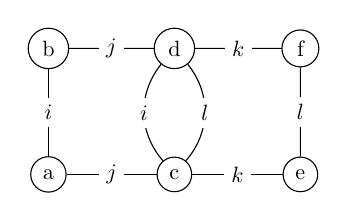
\begin{tikzpicture}[scale=.8]

        \begin{scope}[every node/.style={circle,draw, transform shape}]
          \node (1)  at (0,2)  {b};
          \node (2)  at (0,0)  {a};
          \node (3)  at (2,2)  {d};
          \node (4)  at (2,0)  {c};
          \node (5)  at (4,2)  {f};
          \node (6)  at (4,0)  {e};
        \end{scope}

        \begin{scope}[every node/.style={fill=white, transform shape}]

          \begin{scope}[every edge/.style={draw}]
            \path (1)  edge node {$i$} (2);
            \path (3)  edge[bend right=40] node {$i$} (4);
            \path (1)  edge node {$j$} (3);
            \path (2)  edge node {$j$} (4);
            \path (3)  edge node {$k$} (5);
            \path (4)  edge node {$k$} (6);
            \path (3)  edge[bend left=40] node {$l$} (4);
            \path (5)  edge node {$l$} (6);

          \end{scope}
        \end{scope}

      \end{tikzpicture}
      \caption{}
    \end{center}
  \end{figure}

  \paragraph{}
  If $j$ and $k$ are not consecutive, then an alternating square must be built, it cannot use any of the existing points.

  \begin{figure}[H]
    \begin{center}
      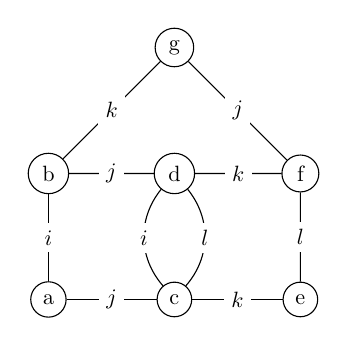
\begin{tikzpicture}[scale=.8]

        \begin{scope}[every node/.style={circle,draw, transform shape}]
          \node (1)  at (0,2)  {b};
          \node (2)  at (0,0)  {a};
          \node (3)  at (2,2)  {d};
          \node (4)  at (2,0)  {c};
          \node (5)  at (4,2)  {f};
          \node (6)  at (4,0)  {e};
          \node (7)  at (2,4)  {g};
        \end{scope}

        \begin{scope}[every node/.style={fill=white, transform shape}]

          \begin{scope}[every edge/.style={draw}]
            \path (1)  edge node {$i$} (2);
            \path (3)  edge[bend right=40] node {$i$} (4);
            \path (1)  edge node {$j$} (3);
            \path (2)  edge node {$j$} (4);
            \path (5)  edge node {$j$} (7);
            \path (3)  edge node {$k$} (5);
            \path (4)  edge node {$k$} (6);
            \path (1)  edge node {$k$} (7);
            \path (3)  edge[bend left=40] node {$l$} (4);
            \path (5)  edge node {$l$} (6);

          \end{scope}
        \end{scope}

      \end{tikzpicture}
      \caption{}
    \end{center}
  \end{figure}

  \paragraph{}
  Thus there is a cycle of length 3. Otherwise $j$ and $k$ are consecutive, thus $j = k+1$ (up to duality).

  \begin{figure}[H]
    \begin{center}
      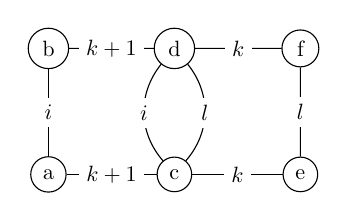
\begin{tikzpicture}[scale=.8]

        \begin{scope}[every node/.style={circle,draw, transform shape}]
          \node (1)  at (0,2)  {b};
          \node (2)  at (0,0)  {a};
          \node (3)  at (2,2)  {d};
          \node (4)  at (2,0)  {c};
          \node (5)  at (4,2)  {f};
          \node (6)  at (4,0)  {e};
        \end{scope}

        \begin{scope}[every node/.style={fill=white, transform shape}]

          \begin{scope}[every edge/.style={draw}]
            \path (1)  edge node {$i$} (2);
            \path (3)  edge[bend right=40] node {$i$} (4);
            \path (1)  edge node {$k+1$} (3);
            \path (2)  edge node {$k+1$} (4);
            \path (3)  edge node {$k$} (5);
            \path (4)  edge node {$k$} (6);
            \path (3)  edge[bend left=40] node {$l$} (4);
            \path (5)  edge node {$l$} (6);

          \end{scope}
        \end{scope}

      \end{tikzpicture}
      \caption{}
    \end{center}
  \end{figure}

  \paragraph{}
  If $i$ and $k$ are not consecutive then a $\rho_i$ edge must be placed between $e$ and $f$. However, by Proposition~\ref{square-connection}, an additionnal square must be built. In order to end the sequence the horizontal component of the squares at the end of the pattern must be adjacent to $i$ or $l$.

  \paragraph{}
  Suppose that we are currently at the left end of a such sequence, then $k+1$ is consecutive to $l$ and $l = k + 2$. The graph is the following one:

  \begin{figure}[H]
    \begin{center}
      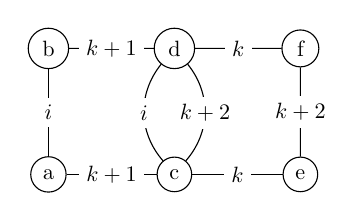
\begin{tikzpicture}[scale=.8]

        \begin{scope}[every node/.style={circle,draw, transform shape}]
          \node (1)  at (0,2)  {b};
          \node (2)  at (0,0)  {a};
          \node (3)  at (2,2)  {d};
          \node (4)  at (2,0)  {c};
          \node (5)  at (4,2)  {f};
          \node (6)  at (4,0)  {e};
        \end{scope}

        \begin{scope}[every node/.style={fill=white, transform shape}]

          \begin{scope}[every edge/.style={draw}]
            \path (1)  edge node {$i$} (2);
            \path (3)  edge[bend right=40] node {$i$} (4);
            \path (1)  edge node {$k+1$} (3);
            \path (2)  edge node {$k+1$} (4);
            \path (3)  edge node {$k$} (5);
            \path (4)  edge node {$k$} (6);
            \path (3)  edge[bend left=40] node {$k+2$} (4);
            \path (5)  edge node {$k+2$} (6);

          \end{scope}
        \end{scope}

      \end{tikzpicture}
      \caption{}
    \end{center}
  \end{figure}

  \paragraph{}
  Because the sequence is not monotone, the vertical component of the last square must be $\rho_{k+2}$.

  \paragraph{}
  If there are 6 points, $i$ and $k$ must be consecutive and thus $k = i+1$. The pattern must be

  \begin{figure}[H]
    \begin{center}
      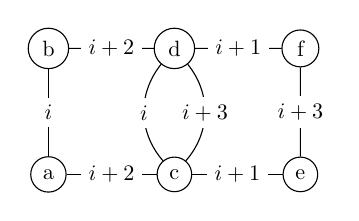
\begin{tikzpicture}[scale=.8]

        \begin{scope}[every node/.style={circle,draw, transform shape}]
          \node (1)  at (0,2)  {b};
          \node (2)  at (0,0)  {a};
          \node (3)  at (2,2)  {d};
          \node (4)  at (2,0)  {c};
          \node (5)  at (4,2)  {f};
          \node (6)  at (4,0)  {e};
        \end{scope}

        \begin{scope}[every node/.style={fill=white, transform shape}]

          \begin{scope}[every edge/.style={draw}]
            \path (1)  edge node {$i$} (2);
            \path (3)  edge[bend right=40] node {$i$} (4);
            \path (1)  edge node {$i+2$} (3);
            \path (2)  edge node {$i+2$} (4);
            \path (3)  edge node {$i+1$} (5);
            \path (4)  edge node {$i+1$} (6);
            \path (3)  edge[bend left=40] node {$i+3$} (4);
            \path (5)  edge node {$i+3$} (6);

          \end{scope}
        \end{scope}

      \end{tikzpicture}
      \caption{}
    \end{center}
  \end{figure}

  \paragraph{}
  Otherwise if there are 8 points, then $k-1$ must be adjacent to $i$ and thus $k = i+2$. The pattern is this one:

  \begin{figure}[H]
    \begin{center}
      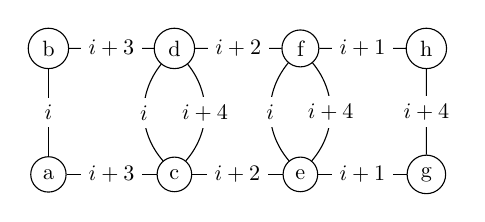
\begin{tikzpicture}[scale=.8]

        \begin{scope}[every node/.style={circle,draw, transform shape}]
          \node (1)  at (0,2)  {b};
          \node (2)  at (0,0)  {a};
          \node (3)  at (2,2)  {d};
          \node (4)  at (2,0)  {c};
          \node (5)  at (4,2)  {f};
          \node (6)  at (4,0)  {e};
          \node (7)  at (6,2)  {h};
          \node (8)  at (6,0)  {g};
        \end{scope}

        \begin{scope}[every node/.style={fill=white, transform shape}]

          \begin{scope}[every edge/.style={draw}]
            \path (1)  edge node {$i$} (2);
            \path (3)  edge[bend right=40] node {$i$} (4);
            \path (5)  edge[bend right=40] node {$i$} (6);
            \path (1)  edge node {$i+3$} (3);
            \path (2)  edge node {$i+3$} (4);
            \path (3)  edge node {$i+2$} (5);
            \path (4)  edge node {$i+2$} (6);
            \path (7)  edge node {$i+1$} (5);
            \path (8)  edge node {$i+1$} (6);
            \path (3)  edge[bend left=40] node {$i+4$} (4);
            \path (5)  edge[bend left=40] node {$i+4$} (6);
            \path (7)  edge node {$i+4$} (8);

          \end{scope}
        \end{scope}

      \end{tikzpicture}
      \caption{}
    \end{center}
  \end{figure}

  \paragraph{}
  If there are 10 points, we are limited because there are only five involutions. Thus the only possible pattern is:

  \begin{figure}[H]
    \begin{center}
      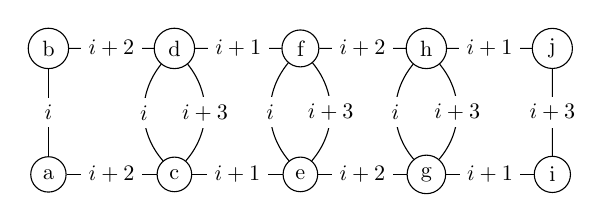
\begin{tikzpicture}[scale=.8]

        \begin{scope}[every node/.style={circle,draw, transform shape}]
          \node (1)  at (0,2)  {b};
          \node (2)  at (0,0)  {a};
          \node (3)  at (2,2)  {d};
          \node (4)  at (2,0)  {c};
          \node (5)  at (4,2)  {f};
          \node (6)  at (4,0)  {e};
          \node (7)  at (6,2)  {h};
          \node (8)  at (6,0)  {g};
          \node (9)  at (8,2)  {j};
          \node (10) at (8,0)  {i};
        \end{scope}

        \begin{scope}[every node/.style={fill=white, transform shape}]

          \begin{scope}[every edge/.style={draw}]
            \path (1)  edge node {$i$} (2);
            \path (3)  edge[bend right=40] node {$i$} (4);
            \path (5)  edge[bend right=40] node {$i$} (6);
            \path (7)  edge[bend right=40] node {$i$} (8);
            \path (1)  edge node {$i+2$} (3);
            \path (2)  edge node {$i+2$} (4);
            \path (3)  edge node {$i+1$} (5);
            \path (4)  edge node {$i+1$} (6);
            \path (9)  edge node {$i+1$} (7);
            \path (10) edge node {$i+1$} (8);
            \path (7)  edge node {$i+2$} (5);
            \path (8)  edge node {$i+2$} (6);
            \path (3)  edge[bend left=40] node {$i+3$} (4);
            \path (5)  edge[bend left=40] node {$i+3$} (6);
            \path (7)  edge[bend left=40] node {$i+3$} (8);
            \path (9)  edge node {$i+3$} (10);

          \end{scope}
        \end{scope}

      \end{tikzpicture}
      \caption{}
    \end{center}
  \end{figure}

  \paragraph{}
  But this pattern contains the pattern displayed in Figure~\ref{linear-1} and thus one of the two patterns is contained in it.

  \paragraph{}
  We can see that no other cycle can be made, even for a bigger number of involutions and a bigger number of points. For a general study of all possible permutation representation graph, it can be useful to enumerate more completly on the possible pattern of this family.

\end{proof}

\begin{corollary}
  \label{even-sequence}
  Every sequence of alternating square (cyclic or non-cyclic) that does not contains any non-linear cycle seen in Proposition~\ref{rotation-pattern} and~\ref{linear-pattern} contains an even number of points.
\end{corollary}

\begin{proof}
  We do not have any of the special patterns. Starting from a square, each added square to the sequence can be added in a linear and monotone fashion and in this case, it use two points. Otherwise it must one of the patterns found in Propositions~\ref{rotation-pattern} and~\ref{linear-pattern} but both of them add an even number of points.
\end{proof}

\begin{proposition}
  \label{sequence-connection}
  A sequence that cannot be extended can only be adjacent to a single edge.
\end{proposition}

\section{General properties}

\begin{proposition}
  \label{patterns-adding}
  When adding edge of an involution $\rho_i$ to an existing permutation representation graph, for each $\rho_j$ that must commute with $\rho_i$, the following patterns are possible:
  \begin{enumerate}
    \item An alternating square $[\rho_i, \rho_j]$.
    \item Two double edges $(\rho_i, \rho_j)$.
    \item One double edge $(\rho_i, \rho_j)$ and a single edge between two points fixed by $\rho_i$.
  \end{enumerate}
\end{proposition}

\begin{proof}
  This is a clear corollary of Property~\ref{intersection-patterns}.
\end{proof}

\paragraph{}
In the next chapter we prove that there are no polytopes of a given rank with automorphism group $A_{11}$. To do this we generate all the possible permutation representation graphs and then prove that, if such a graph exists, the graph is not a string C-group representation of $A_{11}$.

\paragraph{}
To generate all the possible permutation representation graphs we need a single and systematic method. We will use the following one:

\begin{method}
  \label{method}
  This is a method that we used when we want to find all string C-group representations of a given group ($A_{11}$ in our case).

  \paragraph{}
  To achieve this, we start by finding all permutation representation graphs. The following method is applied:

  \begin{enumerate}
    \item Choose an involution and draw the graph with only this involution.
    \item Choose an other involution and use Lemma~\ref{patterns-adding} to create a list of start patterns.
    \item Attach all vertices until the graph is connected. Extra edges can be placed during this step to satisfy various constraints.
    \item Add remaining edges.
  \end{enumerate}

  \paragraph{}
  Once this is done, we must check the sggi that we found is a monodromy group, i.e. that the generating set is free. Then this monodromy group must satisfy the intersection property and is thus a string C-group representation. Finally, we check that the string C-group is a representation of $A_{11}$ and not of one of its transitive subgroup.

\end{method}

\begin{lemma}
  \label{rho0atEnd}
  In permutation representation graph on $n$ vertices, if there are $r < \frac{n}{2}$ $\rho_0$ edges that are not in an alternating square, then there are at least $r$ $\rho_1$ edges that are not in an alternating square.
\end{lemma}

\begin{proof}
  If the $\rho_0$ edges are not part of an alternating square then they must be adjacent to a simple edge, a double edge or an alternating square. But the last two cases are impossible by Propositions~\ref{square-connection} and~\ref{continue-double-edge} because there are no $\rho_{-1}$ involution.

  \paragraph{}
  Moreover, if two $\rho_0$ share a $\rho_1$ edge like in the Figure~\ref{rho0Fig}, then this component needs a $\rho_1$ edge for the same reason.

  \begin{figure}[H]
    \begin{center}
      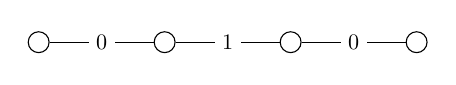
\begin{tikzpicture}[scale=.8]

        \begin{scope}[every node/.style={circle,draw, transform shape}]
          \node (1)  at (0,0)  {};
          \node (2)  at (2,0)  {};
          \node (3)  at (4,0)  {};
          \node (4)  at (6,0)  {};
        \end{scope}

        \begin{scope}[every node/.style={fill=white, transform shape}]

          \begin{scope}[every edge/.style={draw}]
            \path (1)  edge node {$0$} (2);
            \path (3)  edge node {$0$} (4);
            \path (2)  edge node {$1$} (3);
          \end{scope}
        \end{scope}

      \end{tikzpicture}
      \caption{}
      \label{rho0Fig}
    \end{center}
  \end{figure}
\end{proof}
